\input{../latexSetup}

\usepackage{tikz}
\usetikzlibrary{arrows.meta, decorations.pathmorphing}
\usepackage{amssymb}
\usepackage{nicefrac}

\lhead{\Large 33-211}
\chead{\Large Physics 3 : Modern Essentials}
\rhead{\Large Lecture 4}

\begin{document}
\thispagestyle{fancy}

\begin{center}
  {\huge \textbf{The Invariant Interval}}
\end{center}

% ============================================================
\section*{Einstein's Principle of Relativity}

\textbf{\underline{ALL}} laws of physics are the same in every inertial reference frame.

\textit{Inertial} means non-accelerating, not subject to net force.
(See Book for details.)

\textbf{Carefully:} Both the \emph{form} of laws \emph{and} the \emph{numerical values}
of the physical constants.

\medskip
\textbf{Idea:} Choice of particular coordinate system is \underline{arbitrary}.
The laws of physics shouldn't be sensitive to which choice was made.
$\Rightarrow$ The form \& all the constants must be the same.

% ============================================================
\section*{Content of the Principle of Relativity}

\begin{tcolorbox}
With G.T., saw:
\[
  F = \frac{dp}{dt} \quad \text{in } S
  \qquad\Longleftrightarrow\qquad
  F' = \frac{dp'}{dt'} \quad \text{in } S'
\]
This satisfies the PaR, but is even more restrictive.

PaR \emph{only} requires:
\[
  F = \frac{dp}{dt} \quad \text{in } S
  \qquad\text{and}\qquad
  \textcolor{red}{F' \neq \frac{dp'}{dt'}} \quad \text{in } S'
  \quad \leftarrow \textcolor{red}{\text{Ok if not equal}}
\]
\end{tcolorbox}

This is how E\&M can satisfy PaR when $\vec{E}\leftrightarrow\vec{B}$ in the charged-bar example.

% ============================================================
\section*{But One of the Constants is a Speed! $c$.}

How can that not depend on your reference frame?

\begin{center}
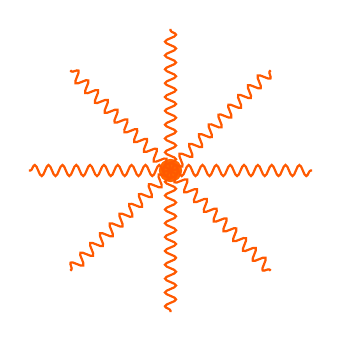
\begin{tikzpicture}[scale=1.0, >=Stealth]
  % Central source (orange dot)
  \filldraw[orange!80!red] (0,0) circle (4pt);
  % 8 wavy rays radiating outward
  \foreach \angle/\label/\pos in {
      90/{Observer 1}/above,
      180/{Observer 2}/left,
      0/{Observer 3}/right,
      225/{}/below left,
      315/{}/below right,
      45/{}/above right,
      270/{}/below,
      135/{}/above left} {
    \draw[orange!70!red, thick,
          decorate, decoration={snake, amplitude=2pt, segment length=5pt}]
      (0,0) -- (\angle:1.8);
  }
\end{tikzpicture}
\hspace{2em}
\begin{minipage}{0.4\textwidth}
  \begin{itemize}
    \item[$\bullet$] Observer 1 (above)
    \item[$\bullet$] Observer 2 ($\leftarrow$)
    \item[$\bullet$] Observer 3 ($\rightarrow$)
  \end{itemize}
  \vspace{0.3em}
  $\left.\rule{0pt}{3em}\right\}$ All measure speed of light $= c$!
\end{minipage}
\end{center}

Saw a preview of how this works with General Coordinate Transforms at $v_*$.
Will now go through it from a different starting point.
\textbf{What must be true if different observers agree on the speed of light?}

% ============================================================
\section*{Warm Up: Geometric Analogy}

Two surveying companies (Engineering and Chemistry) mapped CMU with slightly
different orientations.

\begin{center}
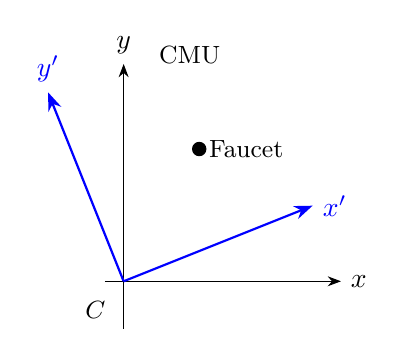
\begin{tikzpicture}[scale=1.2, >=Stealth]
  % Standard axes (Engineering)
  \draw[->] (-0.2,0) -- (2.3,0) node[right] {$x$};
  \draw[->] (0,-0.5) -- (0,2.3) node[above] {$y$};
  \node[font=\small] at (-0.3,-0.3) {$C$};
  % Rotated axes (Chemistry)
  \draw[->, blue, thick] (0,0) -- (2.0,0.8) node[right] {$x'$};
  \draw[->, blue, thick] (0,0) -- (-0.8,2.0) node[above] {$y'$};
  % Particle/point
  \filldraw (0.8,1.4) circle (2pt) node[right, font=\small] {Faucet};
  % Label
  \node[above, font=\small] at (0.7,2.2) {CMU};
\end{tikzpicture}
\end{center}

$x$-coordinate measured in meters; $y$-coordinate measured in \underline{miles}.

\medskip
The companies did detailed, accurate measurements but didn't talk to each other.
One day, an open-minded physics student studied both and took the daring step of
using the \emph{same dimension} for $x$ and $y$ — conversion factor $k$.

Then discovered the quantity:
\[
  \sqrt{x^2 + (ky)^2} = \sqrt{x'^2 + (ky')^2} \equiv \text{Distance}
\]

\textbf{``Discovered principle of invariance of distance''}

% ============================================================
\section*{Relativity: Points $\to$ Events}

In relativity, points become \textbf{events} in Space + time.
(See Book discussion about lattice of synchronized clocks.)
\[
  \text{Event} = (x,\,y,\,z,\,t) \xrightarrow{\;?\;} (x',\,y',\,z',\,t')
\]
where the transformation is due to relative motion along the $x$-axis.

\subsection*{Big Lesson from Geometric Analogy}

It \textbf{pays} to use the \underline{same units} for all coordinates.

Instead of $t$ \;[$t$]=s, use $ct$ \;[$ct$]=m.

\textbf{Will measure time in meters.}
``One meter of time'' = light-meter = time it takes light to travel 1\,m.

\begin{tcolorbox}
  \textbf{Deep:} $c$ is \underline{not} some sacred physical constant.
  Simply a conversion factor s\,$\to$\,m.
  Analogous to $k$ (mile\,$\to$\,m).
\end{tcolorbox}

% ============================================================
\section*{What Do the Coordinate Transforms Have to Be?}

\[
  (ct,\,x,\,y,\,z) \xrightarrow{\;v\;} (ct',\,x',\,y',\,z')
\]
to keep $c$ constant?

\subsubsection*{Start Easy: $y'=y$, $z'=z$}

Direction $\perp$ to relative motion is unaffected.

\begin{center}
\begin{tikzpicture}[scale=1.0, >=Stealth]
  % Axes
  \draw[->] (-0.3,0) -- (3.5,0) node[right] {$x$};
  \draw[->] (0,-0.2) -- (0,2.0) node[above] {};
  \node[left, font=\small] at (0,1.3) {$1$\,m};
  % Tick mark at y=1m
  \draw[thick] (-0.05,1.3) -- (0.05,1.3);
  % Rocket (red box) moving right at y=1m
  \draw[red, thick] (1.3,1.1) -- (1.3,1.5) -- (1.9,1.5) -- (1.9,1.1) -- cycle;
  \draw[red, ->, thick] (1.9,1.3) -- (2.3,1.3) node[right, font=\small] {};
  \node[red, font=\small] at (1.6,1.3) {Pan};
  % Dashed line from rocket to axis
  \draw[red, dashed] (1.6,1.1) -- (1.6,0);
\end{tikzpicture}
\end{center}

``Pan'' marks measure the lab $y$-coordinate of the $y=1$ rocket frame.
In the lab frame the marks will be on $y=1$.
If they weren't, then \textbf{both} observers would agree that the rocket passed
above/below $y=1$ (by looking at the marks!).
This would distinguish the two frames — violates PaR. (Ditto $z$.)

% ============================================================
\section*{The Light Clock}

Can now use invariance of $\perp$ distances as a clean way to \textbf{compare clocks}.

\begin{center}
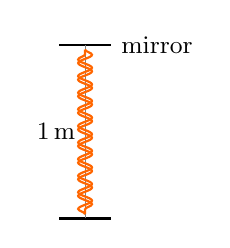
\begin{tikzpicture}[scale=1.1]
  % Mirror at top, base at bottom
  \draw[thick] (-0.3,2.0) -- (0.3,2.0) node[right, font=\small] {mirror};
  \draw[thick] (-0.3,0.0) -- (0.3,0.0);
  % vertical guides
  \draw[thin, gray] (0,0) -- (0,2.0);
  \node[left, font=\small] at (0,1.0) {$1$\,m};
  % Wavy light path (up then down)
  \draw[orange!80!red, thick,
        decorate, decoration={snake, amplitude=2.5pt, segment length=6pt}]
    (0,0.05) -- (0,1.95);
  \draw[orange!80!red, thick,
        decorate, decoration={snake, amplitude=2.5pt, segment length=6pt}]
    (0,1.95) -- (0,0.05);
\end{tikzpicture}
\end{center}

Clock ``ticks'' every time the light flash returns to the origin.

\medskip
Now compare the clocks in the two frames.
Consider events:
\begin{itemize}
  \item $A$ --- emission of light
  \item $B$ --- the 1\textsuperscript{st} ``tick'' (light returns)
\end{itemize}

\begin{center}
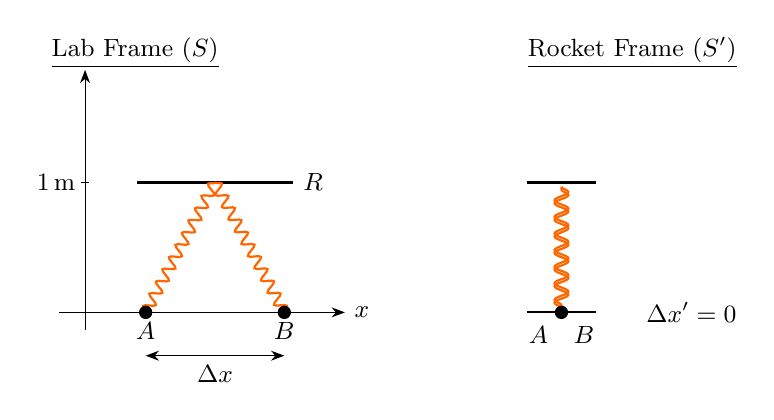
\begin{tikzpicture}[scale=1.1, >=Stealth]

  % === Lab Frame (S) ===
  \begin{scope}[xshift=0cm]
    \node[font=\small, anchor=west] at (-0.5,3.0) {\underline{Lab Frame ($S$)}};
    % Axes
    \draw[->] (-0.3,0) -- (3.0,0) node[right, font=\small] {$x$};
    \draw[->] (0,-0.2) -- (0,2.8);
    \node[left, font=\small] at (0,1.5) {$1$\,m};
    \draw[thin] (-0.05,1.5) -- (0.05,1.5);

    % Mirror (horizontal, at y=1m, between A and B)
    \draw[thick] (0.6,1.5) -- (2.4,1.5) node[right, font=\small] {$R$};

    % Light path: A -> mirror -> B (orange zigzag)
    \draw[orange!80!red, thick,
          decorate, decoration={snake, amplitude=2pt, segment length=5pt}]
      (0.7,0) -- (1.5,1.5);
    \draw[orange!80!red, thick,
          decorate, decoration={snake, amplitude=2pt, segment length=5pt}]
      (1.5,1.5) -- (2.3,0);

    % Events
    \filldraw (0.7,0) circle (2pt);
    \node[below, font=\small] at (0.7,0) {$A$};
    \filldraw (2.3,0) circle (2pt);
    \node[below, font=\small] at (2.3,0) {$B$};

    % Δx label
    \draw[<->, thin] (0.7,-0.5) -- (2.3,-0.5);
    \node[below, font=\small] at (1.5,-0.5) {$\Delta x$};
  \end{scope}

  % === Rocket Frame (S') ===
  \begin{scope}[xshift=5.5cm]
    \node[font=\small, anchor=west] at (-0.5,3.0) {\underline{Rocket Frame ($S'$)}};
    % Mirror
    \draw[thick] (-0.4,1.5) -- (0.4,1.5);
    \draw[thick] (-0.4,0.0) -- (0.4,0.0);
    % Light path: straight up and down
    \draw[orange!80!red, thick,
          decorate, decoration={snake, amplitude=2.5pt, segment length=6pt}]
      (0,0.05) -- (0,1.45);
    \draw[orange!80!red, thick,
          decorate, decoration={snake, amplitude=2.5pt, segment length=6pt}]
      (0,1.45) -- (0,0.05);
    % Events
    \filldraw (0,0) circle (2pt);
    \node[below, font=\small] at (0,-0.05) {$A\quad B$};
    % Δx' = 0
    \node[font=\small] at (1.5,0) {$\Delta x'=0$};
  \end{scope}

\end{tikzpicture}
\end{center}

% ============================================================
\section*{Coordinates of $A$ and $B$}

$A$ happens at $t=t'=0$ when the coordinate systems coincide:
\[
  x_A = 0,\quad t_A = 0, \qquad x'_A = 0,\quad t'_A = 0
\]

\textbf{In the rocket frame} light goes straight up 1\,m and comes back down 1\,m:
\[
  x'_B = 0, \qquad t'_B = 2\,\text{m} \quad (= 2\,\text{m}/c \text{ in seconds})
\]

Difference in coordinates:
\[
  \Delta x' = 0, \qquad \Delta t' = 2\,\text{m}
\]

\textbf{In the lab frame} there is non-zero $\Delta x$ between $A$ and $B$
(the rocket moved while light traveled!).
Large $v \Rightarrow$ large $\Delta x$; \; small $v \Rightarrow$ small $\Delta x$.

\begin{center}
\begin{tikzpicture}[scale=1.3, >=Stealth]
  % Triangle: A at bottom left, B at bottom right, R (mirror) at top center
  \coordinate (A) at (0,0);
  \coordinate (B) at (2.4,0);
  \coordinate (R) at (1.2,1.8);

  % Light paths (orange wavy)
  \draw[orange!80!red, thick,
        decorate, decoration={snake, amplitude=2pt, segment length=5pt}]
    (A) -- (R);
  \draw[orange!80!red, thick,
        decorate, decoration={snake, amplitude=2pt, segment length=5pt}]
    (R) -- (B);

  % Dashed height line
  \draw[dashed] (1.2,0) -- (R);
  \node[right, font=\small] at (1.2,0.9) {$1$\,m};

  % Δx/2 labels on base
  \draw[<->, thin] (0,-0.35) -- (1.2,-0.35);
  \node[below, font=\small] at (0.6,-0.35) {$\Delta x/2$};
  \draw[<->, thin] (1.2,-0.35) -- (2.4,-0.35);
  \node[below, font=\small] at (1.8,-0.35) {$\Delta x/2$};

  % Events
  \filldraw (A) circle (2pt) node[below left, font=\small] {$A$};
  \filldraw (B) circle (2pt) node[below right, font=\small] {$B$};
  \filldraw (R) circle (2pt) node[above, font=\small] {$R$};

  % Total light distance label
  \node[font=\small, align=left] at (4.2,0.9)
    {Light travels\\total distance\\$= 2\times\sqrt{1+\!\left(\tfrac{\Delta x}{2}\right)^{\!2}}$\\[3pt]$>2\,\text{m}$!};
\end{tikzpicture}
\end{center}

% ============================================================
\section*{Time Dilation}

The time difference between $A$ and $B$ is \emph{different} in the two frames:
\[
  \Rightarrow\quad \textbf{Moving clocks tick at different (slower) rates!}
\]

(Before, we just assumed $t=t'$. Now we see it isn't so.)

\begin{center}
\renewcommand{\arraystretch}{1.4}
\begin{tabular}{lcc}
  & \underline{Lab} & \underline{Rocket} \\
  $\Delta x$: & $\Delta x$ & $0$ \\
  $\Delta t$: & $2\sqrt{1+\!\left(\tfrac{\Delta x}{2}\right)^2}$ & $2$ \\
\end{tabular}
\end{center}

The coordinate differences differ between the two frames —
just like $\Delta x\neq\Delta x'$ and $\Delta y\neq\Delta y'$ in the geometry analogy.

\subsubsection*{Note: The Interval}

\begin{align*}
  \Delta t^2 - \Delta x^2
  &= 4\!\left(1+\frac{\Delta x^2}{4}\right) - \Delta x^2 \\
  &= 4 + \Delta x^2 - \Delta x^2 \\
  &= 4 \\
  &= \Delta t'^2 - \Delta x'^2 \;\equiv\; (\text{Interval})^2
\end{align*}

\begin{tcolorbox}
  \textbf{This quantity ``The Interval'' is invariant.}\\
  Coordinate-independent separation between events.\\
  (Analogous to distance in the geometry analogy.)
\end{tcolorbox}

% ============================================================
\section*{Spacetime}

\textbf{\underline{Deep!}} Invariance of the interval implies that time cannot be
separated from space. Space \& time are part of a single entity:

\begin{center}
  {\Large \textbf{Spacetime}}
\end{center}

The geometry of Spacetime is truly 4D (not $3\oplus 1$ as in Newtonian physics).

``The direction of the `time axis' depends on the state of motion of the observer.''

Just like the direction of surveyors' $y$-axis depends on their orientation.

% ============================================================
\section*{Comments}

\begin{itemize}
  \item That $\Delta x$ is different in the two frames is no surprise!
  \item $\Delta t > \Delta t'$ \;--- \textbf{``Moving clocks run slow''}
\[
  \frac{\Delta t}{\Delta t'} = \sqrt{1+\!\left(\frac{\Delta x}{2}\right)^{\!2}} \to 1
  \quad\text{when } \Delta x\to 0 \text{ (small } v\text{)}
\]
\end{itemize}

\begin{center}
\begin{tikzpicture}[scale=1.4, >=Stealth]
  % Isoceles triangle: base = Δx, height = 1m (= Δt'/2), hypotenuse = Δt/2
  \coordinate (TL) at (-1.0,0);
  \coordinate (TR) at ( 1.0,0);
  \coordinate (Top) at (0, 1.6);
  \draw[thick] (TL) -- (Top) -- (TR) -- (TL);
  % Height dashed
  \draw[dashed] (0,0) -- (Top);
  \node[right, font=\small] at (0,0.8) {$1$\,m};
  % Labels on sides
  \node[left,  font=\small] at (-0.55,0.85) {$\Delta t/2$};
  \node[right, font=\small] at ( 0.55,0.85) {$1$\,m$= \Delta t'/2$};
  % Base labels
  \node[below, font=\small] at (-0.5,0) {$\Delta x/2$};
  \node[below, font=\small] at ( 0.5,0) {$\Delta x/2$};
  % Pythagoras
  \node[font=\small, align=left] at (3.0,0.8)
    {$\left(\dfrac{\Delta x}{2}\right)^{\!2} + 1^2 = \left(\dfrac{\Delta t}{2}\right)^{\!2}$\\[6pt]
     $\Delta x^2 + 4 = \Delta t^2$};
\end{tikzpicture}
\end{center}

PaR was used in two ways:
\begin{itemize}
  \item[$-$] $\perp$ distances are the same.
  \item[$-$] $c$ is the same in both frames.
\end{itemize}

% ============================================================
\section*{Compare: Geometry vs.\ Spacetime}

\begin{center}
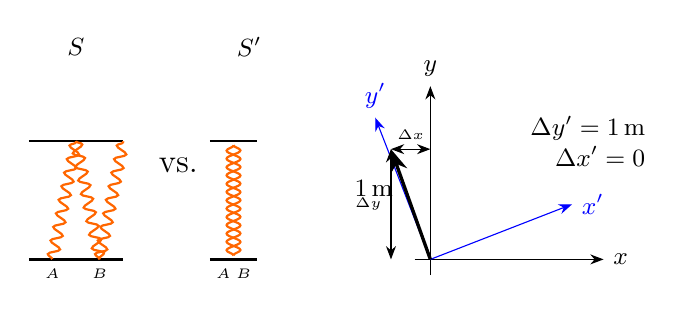
\begin{tikzpicture}[scale=1.0, >=Stealth]
  % Left: two light clocks side by side (Lab S vs Rocket S')
  \begin{scope}[xshift=0cm]
    \node[font=\small] at (0.5,2.7) {$S$};
    \draw[thick] (-0.1,1.5) -- (1.1,1.5);
    \draw[thick] (-0.1,0.0) -- (1.1,0.0);
    % two light paths (two separate ticks)
    \draw[orange!80!red, thick,
          decorate, decoration={snake, amplitude=2pt, segment length=5pt}]
      (0.2,0) -- (0.5,1.5);
    \draw[orange!80!red, thick,
          decorate, decoration={snake, amplitude=2pt, segment length=5pt}]
      (0.5,1.5) -- (0.8,0);
    \draw[orange!80!red, thick,
          decorate, decoration={snake, amplitude=2pt, segment length=5pt}]
      (0.8,0) -- (1.1,1.5);
    \draw[dashed] (0.2,0) -- (0.8,0);
    \node[below, font=\tiny] at (0.2,0) {$A$};
    \node[below, font=\tiny] at (0.8,0) {$B$};
  \end{scope}

  \node[font=\large] at (1.8,1.2) {vs.};

  \begin{scope}[xshift=2.5cm]
    \node[font=\small] at (0.2,2.7) {$S'$};
    \draw[thick] (-0.3,1.5) -- (0.3,1.5);
    \draw[thick] (-0.3,0.0) -- (0.3,0.0);
    \draw[orange!80!red, thick,
          decorate, decoration={snake, amplitude=2.5pt, segment length=6pt}]
      (0,0.05) -- (0,1.45);
    \draw[orange!80!red, thick,
          decorate, decoration={snake, amplitude=2.5pt, segment length=6pt}]
      (0,1.45) -- (0,0.05);
    \node[below, font=\tiny] at (0,0) {$A\;B$};
  \end{scope}

  % Right: geometric analog (rotated axes with 1m vector)
  \begin{scope}[xshift=5.0cm]
    \draw[->] (-0.2,0) -- (2.2,0) node[right, font=\small] {$x$};
    \draw[->] (0,-0.2) -- (0,2.2) node[above, font=\small] {$y$};
    \draw[->, blue] (0,0) -- (1.8,0.7) node[right, font=\small] {$x'$};
    \draw[->, blue] (0,0) -- (-0.7,1.8) node[above, font=\small] {$y'$};
    % 1m vector along y'
    \draw[->, very thick] (0,0) -- (-0.5,1.4);
    \node[left, font=\small] at (-0.35,0.9) {$1$\,m};
    \node[font=\small, align=right] at (2.0,1.5)
      {$\Delta y'=1$\,m\\$\Delta x'=0$};
    % Δx and Δy projections
    \draw[<->, thin] (-0.5,1.4) -- (0,1.4);
    \node[above, font=\tiny] at (-0.25,1.4) {$\Delta x$};
    \draw[<->, thin] (-0.5,0) -- (-0.5,1.4);
    \node[left, font=\tiny] at (-0.5,0.7) {$\Delta y$};
  \end{scope}
\end{tikzpicture}
\end{center}

\begin{center}
\renewcommand{\arraystretch}{1.5}
\begin{tabular}{l|cc|cc}
  & \multicolumn{2}{c|}{\textbf{Geometry}} & \multicolumn{2}{c}{\textbf{Spacetime}} \\
  & $C$ & $C'$ & $S$ & $S'$ \\
  \hline
  Simpler frame? & $C'$ & & $S'$ & \\
  Why? & $\Delta x=0$ & & $\Delta x=0$ & \\
  Simplification & 1 ruler stick needed & & 1 clock needed & \\
  Attention & 2 sticks needed ($x$ \& $y$) & & 2 clocks needed (at $0$ \& $x_B$) & \\
  Complicated because & $\Delta y$ (not full interval!) & & $\Delta t$ (not full interval!) & \\
  & $\Delta y = \sqrt{(AB)^2-(\Delta x)^2} \leq AB$ & &
    $\Delta t = \sqrt{(AB)^2+(\Delta x)^2} \geq AB$ & \\
\end{tabular}
\end{center}

\subsubsection*{Inconsistent?}

\begin{center}
\renewcommand{\arraystretch}{1.4}
\begin{tabular}{p{0.3\textwidth}p{0.3\textwidth}p{0.3\textwidth}}
  & \textbf{Geometry:} identical meter sticks give different $\Delta y$s? &
    \textbf{Spacetime:} identical clocks, different $\Delta t$s? \\
  \hline
  \textbf{No}: & 2 meter sticks in one frame, 1 in the other.
    No $C$ meter stick can be said to disagree w/ $C'$ meter stick. &
    2 clocks vs 1 clock. No lab clock can be said to disagree w/ rocket clock. \\
\end{tabular}
\end{center}

\textbf{Summary:}
\begin{itemize}
  \item No paradox about different $y$-components. Not a fault of meter sticks.
    ``Discrepancy'' from structure of Euclidean Geometry.
  \item No paradox about different time lapses. Not a fault of clocks.
    ``Discrepancy'' from structure of Spacetime.
\end{itemize}

\bigskip
\textbf{HW:} What about a frame $S''$ that is moving faster than $S'$?

\end{document}
